\documentclass[a4paper,11pt]{article}

% --- Paketit ---
\usepackage[utf8]{inputenc}
\usepackage[T1]{fontenc}
\usepackage[finnish]{babel}
\usepackage{amsmath, amssymb, amsthm}
\usepackage{geometry}
\geometry{left=3cm, right=3cm, top=3cm, bottom=3cm}

% --- Grafiikka ja kuvaajat (TikZ & PGFPlots) ---
\usepackage{tikz}
\usetikzlibrary{positioning, automata, arrows.meta, patterns, decorations.pathreplacing}
\usepackage{pgfplots}
\pgfplotsset{compat=1.18}
\usepgfplotslibrary{fillbetween}


% --- Laatikko ---
\usepackage[most]{tcolorbox}

\newtcolorbox{derivationbox}[1][]{
  breakable,                % Sallii laatikon jakautumisen sivunvaihdossa
  enhanced,
  colback=gray!5,          % Hyvin vaalea harmaa tausta
  colframe=gray!50!black,  % Tummanharmaa reunus
  title={#1},              % Otsikko parametrista
  fonttitle=\bfseries\sffamily,
  attach boxed title to top left={yshift=-2mm, xshift=2mm},
  boxed title style={
    colback=gray!50!black,
    sharp corners
  },
  %sharp corners=south,     % Alakulmat terävät
  arc=3mm,                 % Yläkulmat pyöristetyt
  parbox=false             % Sallii tavallisen tekstin ja kaavat
}

% --- Tyyliasetukset ---
\setlength{\parindent}{0pt}
\setlength{\parskip}{1em}
\linespread{1.1}

% --- Otsikointi ---
\title{Optimointimallin matemaattinen johto}
\author{Elias Ervamaa}
\date{\today}

\begin{document}

\maketitle

\section{Johdanto}
Tässä dokumentissa johdetaan analyyttinen ratkaisu kahden jonon resurssien allokointiongelmalle. Tarkastelu etenee kahdessa vaiheessa: ensin johdetaan yksittäisen M/M/1-jonon odotusajan lauseke, minkä jälkeen ratkaistaan optimointiongelma Lagrangen kertoimien menetelmällä.

\subsection{Muuttujat}
Mallissa käytetään seuraavia merkintöjä:
\begin{itemize}
    \item $\lambda_i \in \mathbb{N}$: Saapumisintensiteetti (asiakasta / aikayksikkö).
    \item $\mu_i \in \mathbb{R}_+$: Palvelunopeus (palvelua / aika / työntekijä).
    \item $x_i \in \mathbb{R}_+$: Työntekijöiden määrä.
    \item $w_i \in \mathbb{R}_+$: Odotusajan painokerroin ("haittakerroin").
    \item $c_i \in \mathbb{R}_+$: Työntekijän yksikkökustannus.
    \item $B \in \mathbb{R}_+$: Kokonaisbudjetti.
\end{itemize}

\newpage
\section{Todennäköisyysjakaumat}

\subsubsection*{Saapumisprosessi (Poisson)}
Asiakkaiden saapuminen noudattaa Poisson-prosessia. Todennäköisyys sille, että aikayksikössä ($t$) saapuu tasan $k$ asiakasta, on:
\begin{equation}
    P(X=k) = \frac{\lambda^k e^{-\lambda}}{k!}, \quad k = 0, 1, 2, \dots
\end{equation}

\begin{center}
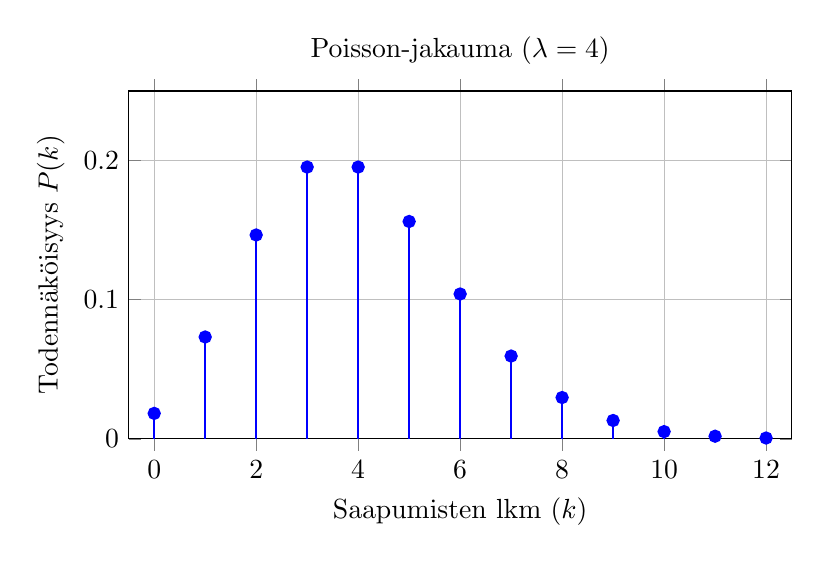
\begin{tikzpicture}
\begin{axis}[
    width=10cm, height=6cm,
    title={Poisson-jakauma ($\lambda=4$)},
    xlabel={Saapumisten lkm ($k$)},
    ylabel={Todennäköisyys $P(k)$},
    ymin=0, ymax=0.25,
    xmin=-0.5, xmax=12.5,
    ybar,
    bar width=2pt,
    grid=major
]
    \addplot+[ycomb, blue, thick, mark=*] coordinates {
        (0, 0.0183) (1, 0.0732) (2, 0.1465) (3, 0.1953) (4, 0.1953)
        (5, 0.1562) (6, 0.1041) (7, 0.0595) (8, 0.0297) (9, 0.0132)
        (10, 0.0052) (11, 0.0019) (12, 0.0006)
    };
\end{axis}
\end{tikzpicture}
\end{center}

\subsubsection*{Palveluajat (Eksponentti)}
Palveluajat $T$ noudattavat eksponenttijakaumaa. Tiheysfunktio on:
\begin{equation}
    f(t; \mu) = \mu e^{-\mu t}, \quad t \ge 0
\end{equation}
Tässä $\mu$ kuvaa palvelunopeutta (rate), joten keskimääräinen palveluaika on $E[T] = 1/\mu$.

\begin{center}
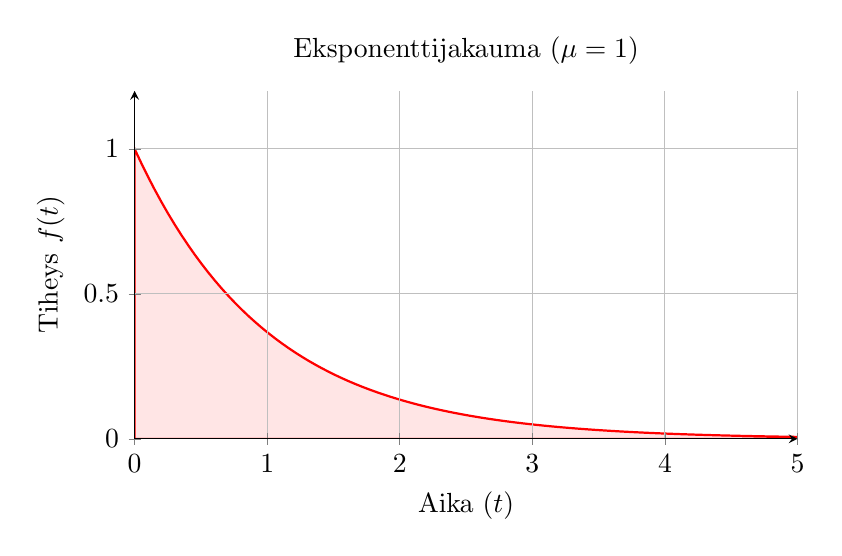
\begin{tikzpicture}
\begin{axis}[
    width=10cm, height=6cm,
    title={Eksponenttijakauma ($\mu=1$)},
    xlabel={Aika ($t$)},
    ylabel={Tiheys $f(t)$},
    domain=0:5, samples=100,
    ymin=0, ymax=1.2,
    axis lines=left,
    grid=major,
    axis on top
]
    \addplot [thick, red, fill=red!10] {exp(-x)} \closedcycle;
\end{axis}
\end{tikzpicture}
\end{center}

\newpage


\section{M/M/1-jonon johtaminen}
\subsection{Tasapainoehto}

% Jotta jono pysyisi tasapainotilassa eikä kasvaisi rajatta, on $x > \frac{\lambda}{\mu}$ (eli $\rho < 1$). Oletetaan, että on kulunut tietty aika, jonka jälkeen jonon jakauma on vakaassa tilassa:

Mallinnetaan yhtä jonoa jatkuva-aikaisena Markov-ketjuna. Systeemin tila $n \in \{0, 1, 2, \dots\}$ kertoo asiakkaiden kokonaismäärän (jonossa + palvelussa).
Systeemin dynamiikka perustuu kahteen voimaan:
\begin{itemize}
    \item \textbf{Saapuminen:} Uusi asiakas saapuu intensiteetillä $\lambda$, mikä nostaa tilaa ($n \to n+1$).
    \item \textbf{Poistuminen:} Palvelu valmistuu intensiteetillä $x\mu$, mikä laskee tilaa ($n \to n-1$). Tämä on mahdollista vain, kun systeemissä on asiakkaita ($n \ge 1$).
\end{itemize}

Määritellään liikennekuorma $\rho = \frac{\lambda}{x\mu}$.
Systeemin stabiilisuus vaatii ehdon $x > \frac{\lambda}{\mu}$ (eli $\rho < 1$).
Oletetaan, että systeemi on ollut toiminnassa riittävän kauan, jolloin alkutilanteen vaikutus on hävinnyt ja systeemi on saavuttanut stokastisen tasapainon. Tämä tapahtuu koska $\rho < 1$, jono ei kasva äärettömyyksiin, vaan todennäköisyysjakauma $p_n$ stabiloituu ajasta riippumattomaksi vakiojakaumaksi. Tässä vakaassa tilassa todennäköisyysvirta tilojen välillä tasaantuu: pitkällä aikavälillä keskimääräinen siirtymä mihin tahansa tilaan $n$ täytyy olla yhtä suuri kuin siirtymä sieltä pois.

Voimme visualisoida tämän tilakaaviona, jossa ympyrät kuvaavat tiloja ja nuolet siirtymäintensiteettejä:



\begin{center}
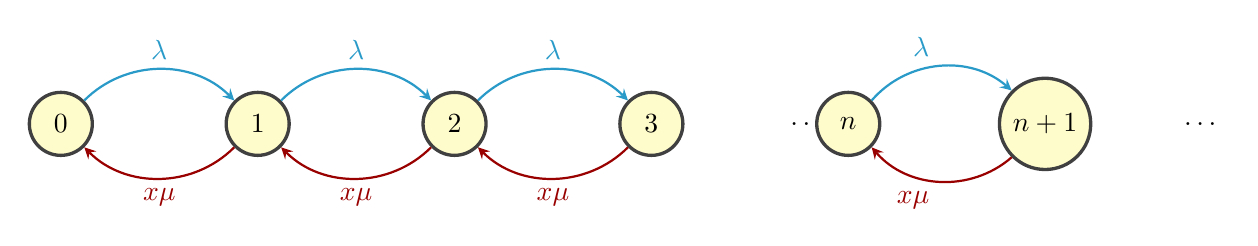
\begin{tikzpicture}[>=stealth, node distance=2.5cm, on grid, auto, initial text=, initial where=left]
    % Tyylit
    \tikzstyle{state}=[circle, draw=black!75, fill=yellow!20, very thick, minimum size=8mm]
    \tikzstyle{arrow}=[->, thick, draw=blue!50!black]

    % Tilat (Solmut)
    \node[state] (0) {0};
    \node[state] (1) [right=of 0] {1};
    \node[state] (2) [right=of 1] {2};
    \node[state] (3) [right=of 2] {3};
    \node (4) [right=of 3, xshift=-0.5cm] {$\dots$}; % Pisteet
    \node[state] (k) [right=of 3] {$n$};
    \node[state] (k1) [right=of k] {$n+1$};
    \node (end) [right=of k1, xshift=-0.5cm] {$\dots$};

    % Siirtymät (Nuolet)
    % Lambda (oikealle)
    \draw[arrow, cyan!80!black] (0) edge [bend left=45] node {$\lambda$} (1);
    \draw[arrow, cyan!80!black] (1) edge [bend left=45] node {$\lambda$} (2);
    \draw[arrow, cyan!80!black] (2) edge [bend left=45] node {$\lambda$} (3);
    \draw[arrow, cyan!80!black] (k) edge [bend left=45] node {$\lambda$} (k1);

    % Mu (vasemmalle) - Huom: mallissa teho on x*mu
    \draw[arrow, red!60!black] (1) edge [bend left=45] node {$x\mu$} (0);
    \draw[arrow, red!60!black] (2) edge [bend left=45] node {$x\mu$} (1);
    \draw[arrow, red!60!black] (3) edge [bend left=45] node {$x\mu$} (2);
    \draw[arrow, red!60!black] (k1) edge [bend left=45] node {$x\mu$} (k);

\end{tikzpicture}
\end{center}

Tarkastellaan leikkausta kahden tilan välissä. Jotta tilannetta kuvaava todennäköisyysjakauma $p_n$ pysyisi vakiona, täytyy virran leikkauksen yli oikealle olla yhtä suuri kuin virran vasemmalle.
Tästä saamme \textbf{globaalin tasapainoyhtälön}:

\begin{equation*}
    \underbrace{\lambda \cdot p_n}_{\text{Virta ylös } (n \to n+1)} = \underbrace{x\mu \cdot p_{n+1}}_{\text{Virta alas } (n+1 \to n)}
\end{equation*}

\textbf{Erikoistapaus}
Systeemi siirtyy tyhjästä (0) tilaan (1) intensiteetillä $\lambda$. Paluu tapahtuu intensiteetillä $x\mu$. Tasapainoehto on:
\begin{equation*}
    \lambda p_0 = x\mu p_1 \implies p_1 = \frac{\lambda}{x\mu} p_0 = \rho p_0 \tag*{(\text{globaali ehto pätee!})}
\end{equation*}

\subsection{Yleinen jäsen}

Saamme rekursiokaavan $p_n = \rho p_{n-1}$, joka sitoo jokaisen tilan edelliseen. 
\begin{align*}
    n=1: \quad p_1 &= \rho p_0 \\
    n=2: \quad p_2 &= \rho p_1 = \rho(\rho p_0) = \rho^2 p_0 \\
    n=3: \quad p_3 &= \rho p_2 = \rho(\rho^2 p_0) = \rho^3 p_0 \\
    &\vdots \\
    \text{Yleisesti: } \quad p_n &= \rho^n p_0
\end{align*}

\begin{derivationbox}
\begin{proof}
    \textbf{Alkuaskel:} \\
    Kun $n=0$, saamme $\rho^0 p_0 = 1 \cdot p_0 = p_0$, tosi.

    \textbf{Induktio-oletus:} \\
    Oletetaan, että väite on tosi mielivaltaisella arvolla $n=k$, eli $p_k = \rho^k p_0$.

    \textbf{Induktioaskel:} \\
    Tarkastellaan arvoa $n=k+1$. Tasapainoyhtälön mukaan:
    \begin{equation*}
        p_{k+1} = \rho \cdot p_k
    \end{equation*}
    Sijoitetaan tähän induktio-oletus $p_k$:n paikalle:
    \begin{equation*}
        p_{k+1} = \rho \cdot (\rho^k p_0) = \rho^{k+1} p_0
    \end{equation*}
    Tämä vastaa väitettä arvolla $n=k+1$.

    \textbf{Päätös:} \\
    Kaava $p_n = \rho^n p_0$ pätee kaikilla kokonaisluvuilla $n \ge 0$.
\end{proof}
\end{derivationbox}


\subsection{Jakauman johtaminen}
Saimme yleisen termin $p_n = \rho^n p_0$. Koska todennäköisyyksien summan täytyy olla 1, voimme ratkaista tuntemattoman vakion $p_0$:


\begin{equation*}
    \sum_{n=0}^{\infty} p_n = p_0 \sum_{n=0}^{\infty} \rho^n = 1
\end{equation*}

Kun stabiilisuusehto $\rho < 1$ on voimassa, geometrinen sarja suppenee arvoon $\frac{1}{1-\rho}$.
\begin{equation*}
    p_0 \cdot \frac{1}{1-\rho} = 1 \implies p_0 = 1 - \rho
\end{equation*}

Sijoittamalla $p_0$ takaisin yleiseen termiin saamme lopullisen todennäköisyysjakauman:
\begin{equation*} \label{eq:pn_distribution}
    p_n = (1-\rho)\rho^n
\end{equation*}





\begin{center}
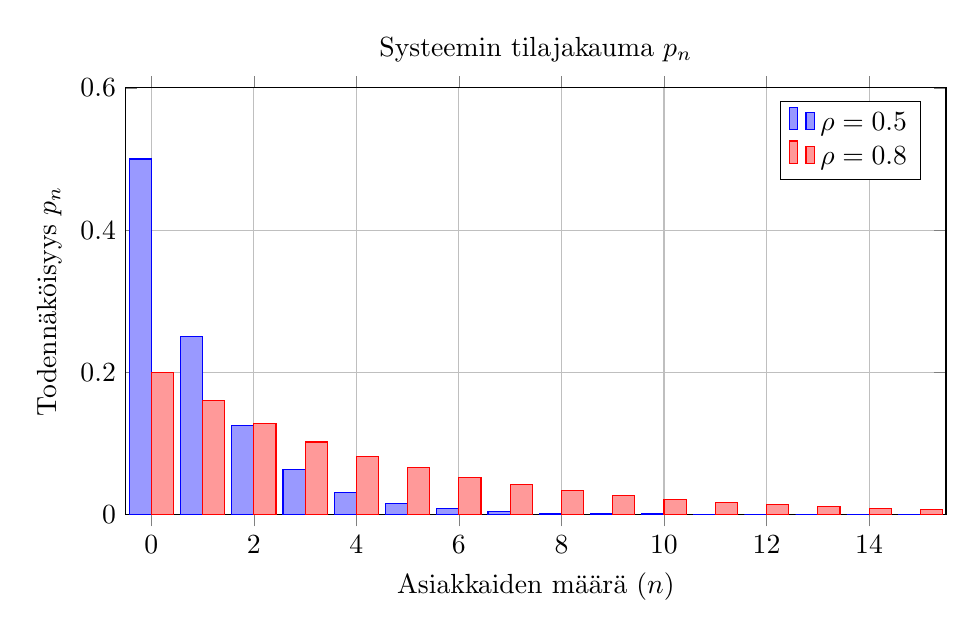
\begin{tikzpicture}
\begin{axis}[
    width=12cm, height=7cm,
    title={Systeemin tilajakauma $p_n$},
    xlabel={Asiakkaiden määrä ($n$)},
    ylabel={Todennäköisyys $p_n$},
    xmin=-0.5, xmax=15.5,
    ymin=0, ymax=0.6,
    ybar=0pt,
    bar width=8pt,
    legend pos=north east,
    grid=major
]
    % Tapaus 1: Rho = 0.5
    \addplot[fill=blue!40, draw=blue] coordinates {
        (0,0.500) (1,0.250) (2,0.125) (3,0.063) (4,0.031)
        (5,0.016) (6,0.008) (7,0.004) (8,0.002) (9,0.001)
        (10,0.001) (11,0.000) (12,0.000) (13,0.000) (14,0.000) (15,0.000)
    };
    \addlegendentry{$\rho = 0.5$}

    % Tapaus 2: Rho = 0.8
    \addplot[fill=red!40, draw=red] coordinates {
        (0,0.200) (1,0.160) (2,0.128) (3,0.102) (4,0.082)
        (5,0.066) (6,0.052) (7,0.042) (8,0.034) (9,0.027)
        (10,0.021) (11,0.017) (12,0.014) (13,0.011) (14,0.009) (15,0.007)
    };
    \addlegendentry{$\rho = 0.8$}
    
\end{axis}
\end{tikzpicture}
\end{center}





\subsection{Odotettu asiakasmäärä $L$}

Olkoon satunnaismuuttuja $N$ asiakkaiden lukumäärä systeemissä. Äsken johdettu $p_n$ on muuttujan $N$ todennäköisyysfunktio, eli $P(N=n) = p_n$.
Odotusarvo lasketaan summaamalla jokainen tila painotettuna niiden todennäköisyyksillä:
\begin{equation*}
    L = E[N] = \sum_{n=0}^{\infty} n p_n = (1-\rho) \sum_{n=0}^{\infty} n \rho^n
\end{equation*}

Summan $\sum n \rho^n$ laskemiseksi tarkastellaan tuttua geometrista sarjaa funktiota:
\begin{equation*}
    \sum_{n=0}^{\infty} x^n = \frac{1}{1-x}, \quad |x| < 1
\end{equation*}
Derivoidaan yhtälö puolittain muuttujan $x$ suhteen:
\begin{align*}
    \frac{d}{dx} \sum_{n=0}^{\infty} x^n &= \frac{d}{dx} (1-x)^{-1} \\
    \sum_{n=1}^{\infty} n x^{n-1} &= (-1)(1-x)^{-2}(-1) = \frac{1}{(1-x)^2}
\end{align*}
Kerrotaan puolittain $x$:llä, jolloin saadaan haluttu muoto:
\begin{equation*}
    \sum_{n=1}^{\infty} n x^n = \frac{x}{(1-x)^2}
\end{equation*}

Sijoitetaan tämä tulos (missä $x=\rho$) alkuperäiseen odotusarvon lausekkeeseen:
\begin{align*}
    L &= (1-\rho) \cdot \frac{\rho}{(1-\rho)^2} \\
    L &= \frac{\rho}{1-\rho}
\end{align*}

Palautetaan alkuperäiset muuttujat sijoittamalla $\rho = \frac{\lambda}{x\mu}$:
\begin{equation*}
    L(x) = \frac{\frac{\lambda}{x\mu}}{1 - \frac{\lambda}{x\mu}} = \frac{\lambda}{x\mu - \lambda}
\end{equation*}

Eli odotettu asiakasmäärä on: $\frac{\lambda}{x\mu - \lambda}$


\subsection{Odotusaika $W$}

Olemme johtaneet jonon keskimääräisen työntekijämäärästä riippuvan pituuden $L(x)$. Asiakkaan näkökulmasta relevantimpi suure on kuitenkin odotusaika $W$, eli aika, joka kuluu jonottamiseen ja palveluun yhteensä.

Stabiilissa systeemissä pätee Littlen Laki, joka sitoo keskimääräisen lukumäärän ja viipymän toisiinsa saapumisintensiteetin kautta:
\begin{equation*}
    L = \lambda W
\end{equation*}

Ratkaistaan odotusaika $W(x)$ jakamalla aiemmin johdettu $L(x)$ saapumisintensiteetillä $\lambda$:
\begin{equation*} \label{eq:wait_time}
    W(x) = \frac{L(x)}{\lambda} = \frac{1}{\lambda} \cdot \frac{\lambda}{x\mu - \lambda} = \frac{1}{x\mu - \lambda}
\end{equation*}



\subsubsection*{Konveksisuustarkastelu}

Optimoinnin onnistumisen kannalta on kriittistä varmistaa, että odotusaikafunktio $W(x)$ on konveksi muuttujan $x$ suhteen. Tarkastellaan funktion toista derivaattaa:

\begin{align*}
    W(x) &= (x\mu - \lambda)^{-1} \\
    W'(x) &= -1 \cdot (x\mu - \lambda)^{-2} \cdot \mu = -\frac{\mu}{(x\mu - \lambda)^2} \\
    W''(x) &= -(-2) \cdot (x\mu - \lambda)^{-3} \cdot \mu \cdot \mu = \frac{2\mu^2}{(x\mu - \lambda)^3}
\end{align*}

Stabiilisuusehdon nojalla tiedämme, että $x > \lambda/\mu$, jolloin termi $(x\mu - \lambda)$ on positiivinen.
Koska myös osoittaja $2\mu^2$ on aina positiivinen, pätee koko määrittelyjoukossa:
\begin{equation*}
    W''(x) > 0 \tag*{(\text{W on konveksi})}
\end{equation*}







\newpage

\section{Optimointiongelma}

\subsection{Karush-Kuhn-Tucker-ehdot}
Tavoitteena on minimoida kahden jonon ($i=1, 2$) painotettu yhteenlaskettu odotusaika budjettirajoitteella.
Välttämätön oletus: budjetti $B$ on riittävä kattamaan minimistabilisuuden (eli $B > \sum c_i \frac{\lambda_i}{\mu_i}$).

Tarkastellaan minimointiongelmaa, jossa on kaksi epäyhtälörajoitetta: budjettirajoite $h(x)$ ja stabiilisuusrajoitteet $g_i(x)$.

\begin{align*}
    \min \quad & f(x) = \sum_{i=1}^2 \frac{w_i}{x_i \mu_i - \lambda_i} \\
    \text{ehdoilla:} \quad & h(x) = \sum_{i=1}^2 c_i x_i - B \le 0 \quad (\text{Budjetti}) \\
    & g_i(x) = \frac{\lambda_i}{\mu_i} - x_i \le 0 \quad (\text{Stabiilisuus}, \forall i)
\end{align*}

Muodostetaan Lagrangen funktio, jossa $\alpha$ on budjettirajoitteen kertoja ja $\beta_i$ ovat stabiilisuusrajoitteiden kertoimet:
\begin{equation*}
    \mathcal{L}(x, \alpha, \beta) = f(x) + \alpha h(x) + \sum_{i=1}^2 \beta_i g_i(x)
\end{equation*}

Optimipisteessä $x^*$ ja kertoimilla $\alpha, \beta$ on oltava voimassa seuraavat ehdot:

\begin{enumerate}
    \item \textbf{Stationaarisuus} \\
    Gradienttien summa on nolla.
    \begin{equation*}
        \nabla f(x^*) + \alpha \nabla h(x^*) + \sum_{i=1}^2 \beta_i \nabla g_i(x^*) = 0
    \end{equation*}
    
    \item \textbf{Komplementaarinen löysyys} \\
    Kertojan ja rajoitteen tulon on oltava nolla.
    \begin{align*}
        \alpha \cdot h(x^*) &= 0 \\
        \beta_i \cdot g_i(x^*) &= 0 \quad (\forall i)
    \end{align*}
    
    \item \textbf{Pääongelman kelvollisuus} \\
    \begin{equation*}
        h(x^*) \le 0, \quad g_i(x^*) \le 0
    \end{equation*}
    
    \item \textbf{Duaaliongelman kelvollisuus} \\
    \begin{equation*}
        \alpha \ge 0, \quad \beta_i \ge 0
    \end{equation*}
\end{enumerate}


\subsection{Yhtälöryhmän ratkaisu}

KKT-ehdot muodostavat yhtälöryhmän, joka ratkaistaan usein päättelemällä ensin, mitkä rajoitteet ovat aktiivisia (eli yhtä suuria kuin nolla) ja mitkä passiivisia (pienempiä kuin nolla).

\textbf{Stabiilisuusrajoitteiden eliminointi} \\
Tarkastellaan ensin stabiilisuusehtoa $g_i(x) \le 0$. Tavoitefunktio $f(x)$ kasvaa äärettömäksi, kun lähestytään stabiilisuusrajaa ($\lambda_i/\mu_i$). Koska haemme minimiä, optimipiste $x^*$ asettuu väistämättä kauas tästä rajasta, eli stabiilisuusalueen sisäpisteeseen.
Tällöin pätee $g_i(x^*) < 0$.
\begin{itemize}
    \item \textbf{Primaalikelpoisuus (3):} Ehto $g_i \le 0$ toteutuu aidosti.
    \item \textbf{Komplementaarisuus (2):} Koska rajoite on aidosti negatiivinen, on sen kertoimen oltava nolla: $\beta_i = 0$.
\end{itemize}
Tämän seurauksena stabiilisuustermit poistuvat stationaarisuusyhtälöstä.

\textbf{Budjettirajoitteen aktiivisuus ja kertoimen $\alpha$ merkki} \\
Kun $\beta_i=0$, stationaarisuusehto (Ehto 1) yksinkertaistuu muotoon:
\begin{equation*}
    \nabla f(x^*) + \alpha \nabla h(x^*) = 0
\end{equation*}
Tutkitaan gradienttien suuntia osittaisderivaattojen avulla:
\begin{align*}
    \frac{\partial f}{\partial x_i} &= -\frac{w_i \mu_i}{(x_i \mu_i - \lambda_i)^2} \quad (< 0, \text{ koska } w, \mu > 0) \\
    \frac{\partial h}{\partial x_i} &= c_i \quad (> 0, \text{ koska hinnat } > 0)
\end{align*}
Sijoitetaan nämä stationaarisuusehtoon:
\begin{equation*}
    \underbrace{\frac{\partial f}{\partial x_i}}_{(-)} + \alpha \underbrace{\frac{\partial h}{\partial x_i}}_{(+)} = 0
\end{equation*}
Jotta negatiivinen ja positiivinen termi voisivat kumota toisensa nollaksi, on kertoimen $\alpha$ oltava aidosti positiivinen ($\alpha > 0$).

Tästä seuraa:
\begin{itemize}
    \item \textbf{Duaalikelpoisuus (4):} Vaatimus $\alpha \ge 0$ toteutuu, koska löysimme, että $\alpha > 0$.
    \item \textbf{Budjetin käyttö (2):} Koska $\alpha \neq 0$, komplementaarisuusehto vaatii, että $h(x^*) = 0$.
\end{itemize}
Tämä tarkoittaa, että primaalikelpoisuus (3) budjetille toteutuu yhtäsuuruutena:
\begin{equation*}
    \sum c_i x_i^* - B = 0 \implies \sum c_i x_i^* = B
\end{equation*}

\textbf{Muuttujien ratkaiseminen stationaarisuusehdosta} \\
Nyt kun tiedämme, että $\alpha > 0$, voimme ratkaista resurssit $x_i$ sen funktiona. Kirjoitetaan gradienttiyhtälö auki:
\begin{equation*}
    \frac{-w_i \mu_i}{(x_i \mu_i - \lambda_i)^2} + \alpha c_i = 0
\end{equation*}
Siirretään termit ja ratkaistaan $x_i$:
\begin{equation*}
    (x_i \mu_i - \lambda_i)^2 = \frac{w_i \mu_i}{c_i \alpha} \implies x_i = \frac{\lambda_i}{\mu_i} + \frac{1}{\mu_i \sqrt{\alpha}} \sqrt{\frac{w_i \mu_i}{c_i}}
\end{equation*}

\textbf{Kertoimen $\alpha$ eliminointi ja tulkinta} \\
Meillä on nyt lauseke $x_i$:lle, mutta se riippuu tuntemattomasta $\alpha$. Käytetään tietoa, että koko budjetti kuluu.
Sijoitetaan $x_i$:n lauseke budjettiyhtälöön:
\begin{equation*}
    \sum_{i=1}^2 c_i \left( \frac{\lambda_i}{\mu_i} + \frac{1}{\mu_i \sqrt{\alpha}} \sqrt{\frac{w_i \mu_i}{c_i}} \right) = B
\end{equation*}
Avataan summa kahteen osaan:
\begin{equation*}
    \sum_{i=1}^2 \frac{c_i \lambda_i}{\mu_i} + \frac{1}{\sqrt{\alpha}} \sum_{i=1}^2 \frac{c_i}{\mu_i} \sqrt{\frac{w_i \mu_i}{c_i}} = B
\end{equation*}
Ensimmäinen termi $\sum \frac{c_i \lambda_i}{\mu_i}$ kuvaa kustannusta, joka vaaditaan pelkästään jonojen pitämiseen stabiilina (minimiresurssit). Merkitään tätä selkeyden vuoksi symbolilla $B_{min}$.
\begin{equation*}
    B_{min} = \sum_{i=1}^2 \frac{c_i \lambda_i}{\mu_i}
\end{equation*}

Nyt yhtälö sievenee muotoon:
\begin{align*}
    \sum_{i=1}^2 \frac{c_i \lambda_i}{\mu_i} + \frac{1}{\sqrt{\alpha}} \sum_{i=1}^2 \frac{c_i}{\mu_i} \sqrt{\frac{w_i \mu_i}{c_i}} &= B \\
    B_{min} + \frac{1}{\sqrt{\alpha}} \sum_{i=1}^2 \sqrt{\frac{c_i^2 \cdot w_i \mu_i}{\mu_i^2 \cdot c_i}} &= B \\
    B_{min} + \frac{1}{\sqrt{\alpha}} \sum_{i=1}^2 \sqrt{\frac{w_i c_i}{\mu_i}} &= B
\end{align*}

Tästä voimme ratkaista termin $1/\sqrt{\alpha}$, joka kuvaa budjetin jakosuhdetta:
\begin{equation*}
    \frac{1}{\sqrt{\alpha}} = \frac{B - B_{min}}{\sum_{j=1}^2 \sqrt{\frac{w_j c_j}{\mu_j}}}
\end{equation*}
Lopuksi sijoitamme tämän takaisin vaiheessa 3 johdettuun $x_i$:n lausekkeeseen. Saamme:
\begin{equation*}
    x_i^* = \frac{\lambda_i}{\mu_i} + \frac{1}{\mu_i} \sqrt{\frac{w_i \mu_i}{c_i}} \left( \frac{B - B_{min}}{\sum_{j=1}^2 \sqrt{\frac{w_j c_j}{\mu_j}}} \right)
\end{equation*}    


\subsection{Optimaalisuuden riittävyys}

Edellä johdettu ratkaisu $x^*$ perustuu KKT-ehtojen välttämättömyyteen. Jotta voimme varmistua siitä, että kyseessä on aidosti tavoitefunktion minimoiva ratkaisu, on tarkasteltava ongelman konveksisuutta.

Optimointiteorian perustuloksen mukaan KKT-ehdot ovat riittäviä globaalille optimille, mikäli optimointitehtävä on konveksi. Tässä tapauksessa ehdot täyttyvät:

\begin{itemize}
    \item \textbf{Kohdefunktion konveksisuus:} Osoitimme aiemmin toisen derivaatan tarkastelulla, että odotusaikafunktio $W(x_i)$ on aidosti konveksi ($W'' > 0$) koko määrittelyalueellaan. Kahden konveksin funktion summa $f(x)$ on edelleen konveksi.
    \item \textbf{Rajoitejoukon konveksisuus:} Budjettirajoite $h(x)$ ja stabiilisuusrajoitteet $g_i(x)$ ovat lineaarisia (affiineja) funktioita. Lineaariset epäyhtälöt rajaavat aina konveksin joukon (puoliavaruuksien leikkaus).
\end{itemize}

Koska minimoimme konveksia funktiota konveksissa joukossa, löydetty KKT-piste $x^*$ on ongelman yksikäsitteinen \textbf{globaali minimi}.



\newpage
\section{Lopputulos}

\subsection{Analyyttinen ratkaisu}

Optimointiongelman ratkaisuna saamme analyyttisen kaavan optimaaliselle resurssimäärälle $x_i^*$ jokaiselle jonolle $i$. Ratkaisu voidaan esittää muodossa:

\begin{derivationbox}
\begin{equation*} \label{eq:final_result}
    x_i^* = \underbrace{\frac{\lambda_i}{\mu_i}}_{\text{Minimitarve}} + \underbrace{\frac{\sqrt{w_i / c_i \mu_i}}{\sum_{j} \sqrt{w_j c_j / \mu_j}}}_{\text{Allokaatiosuhde}} \cdot \underbrace{\left( B - B_{min} \right)}_{\text{Ylijäämäbudjetti}}
\end{equation*}  
Missä $B_{min} = \sum \frac{c_j \lambda_j}{\mu_j}$ on stabiilisuuden vaatima minimibudjetti.
\end{derivationbox}


\subsection{Tulkinta:}

Kaava (\ref{eq:final_result}) tunnetaan jonoteoriassa ja palveluoperaatioiden johtamisessa nimellä \textit{Square Root Staffing Principle}. Se jakaa resurssit kahteen komponenttiin:
\begin{enumerate}
    \item \textbf{Stabiilisuuskomponentti:} Jokaiselle jonolle on ensin annettava sen liikennekuormaa vastaava määrä resursseja ($\rho = 1$), jotta jono ei kasva äärettömäksi.
    \item \textbf{Optimointikomponentti:} Kun minimitarve on tyydytetty, jäljelle jäävä budjetti jaetaan jonojen kesken. Jakosuhde ei ole suoraan verrannollinen painoarvoihin $w_i$, vaan neliöjuuritermiin $\sqrt{w_i}$.
\end{enumerate}

Tämä tarkoittaa, että jos jonon 1 tärkeyskerroin $w_1$ nelinkertaistuu, se ei saa nelinkertaista määrää lisäresursseja, vaan ainoastaan kaksinkertaisen määrän suhteessa muihin. Tämä vaimennettu reaktio johtuu jonotusteorian konveksisuudesta: ensimmäiset lisäresurssit tuovat suurimman hyödyn, mutta hyöty vähenee resurssien kasvaessa.

\newpage
\subsection{Numeerinen havainnollistaminen}

Tarkastellaan esimerkkitilannetta, jossa meillä on kaksi jonoa. Jono 1 on kriittinen ($w_1=4$) ja Jono 2 on normaali ($w_2=1$). Muut parametrit ovat identtiset ($\lambda=5, \mu=1, c=1$).
Minimibudjetti stabiilisuudelle on $5+5=10$ yksikköä.

Kuvaaja osoittaa, kuinka optimaalinen miehitys $x_i$ muuttuu kokonaisbudjetin $B$ kasvaessa.

\begin{center}
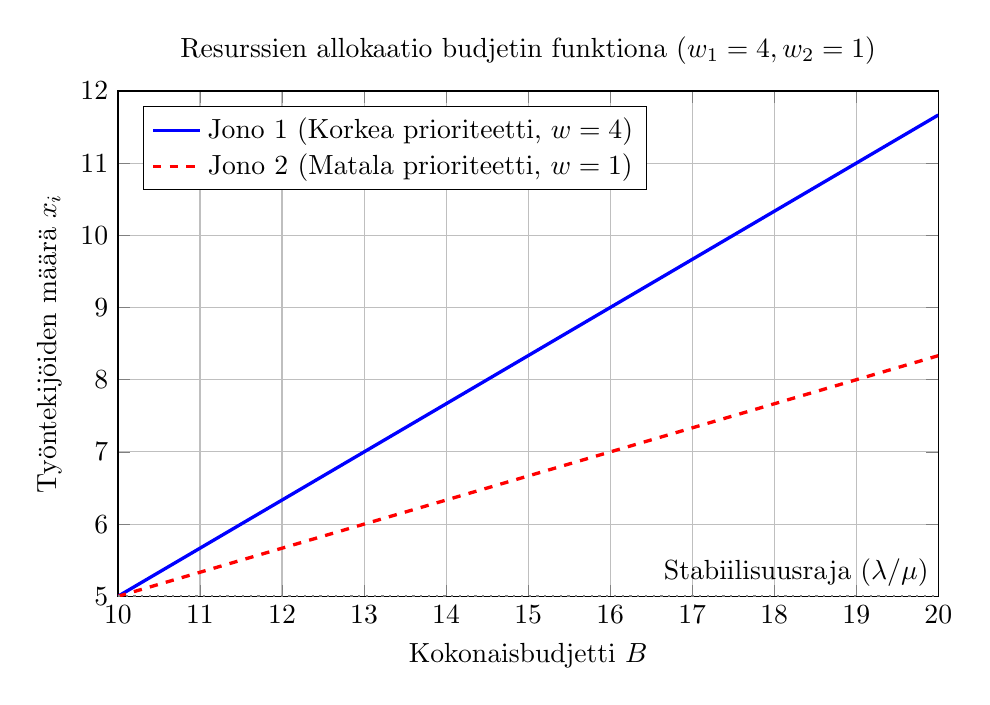
\begin{tikzpicture}
\begin{axis}[
    width=12cm, height=8cm,
    title={Resurssien allokaatio budjetin funktiona ($w_1=4, w_2=1$)},
    xlabel={Kokonaisbudjetti $B$},
    ylabel={Työntekijöiden määrä $x_i$},
    xmin=10, xmax=20,
    ymin=5, ymax=12,
    grid=major,
    legend pos=north west,
    domain=10:20,
    samples=50
]
    % Parametrit selityksenä (näkymätön laskentaan):
    % Lambda = 5, Mu = 1 -> Minimi x = 5.
    % B_min = 10.
    % w1 = 4 -> sqrt(4) = 2.
    % w2 = 1 -> sqrt(1) = 1.
    % Jakaja = 2 + 1 = 3.
    % x1_extra_osuus = 2/3.
    % x2_extra_osuus = 1/3.

    % Jono 1 (Painotettu, w=4)
    % Kaava: 5 + (2/3)*(x - 10)
    \addplot[blue, very thick] {5 + (2/3)*(x - 10)};
    \addlegendentry{Jono 1 (Korkea prioriteetti, $w=4$)}

    % Jono 2 (Normaali, w=1)
    % Kaava: 5 + (1/3)*(x - 10)
    \addplot[red, very thick, dashed] {5 + (1/3)*(x - 10)};
    \addlegendentry{Jono 2 (Matala prioriteetti, $w=1$)}

    % Minimitaso
    \draw[gray, dotted, thick] (axis cs:10, 5) -- (axis cs:20, 5);
    \node[anchor=south east] at (axis cs:20, 5) {Stabiilisuusraja ($\lambda/\mu$)};

\end{axis}
\end{tikzpicture}
\end{center}

Kuvaajasta nähdään selvästi teoreettinen tulos:
\begin{itemize}
    \item Kun $B=10$ (minimibudjetti), molemmat jonot ovat juuri ja juuri stabiileja ($x_1=x_2=5$).
    \item Kun budjetti ylittää minimin, ylijäämä jaetaan jonojen kesken suhteessa painokertoimien neliöjuuriin ($\sqrt{w_i}$). Tässä esimerkissä suhde on $\sqrt{4} : \sqrt{1} = 2 : 1$.
\end{itemize}


\newpage
\section{Teoreettinen verrokki simulaatiolle}

Jotta voimme myöhemmin verrata tuloksia simulaation tuloksiin, laskemme tarkan teoreettisen optimin seuraavalle esimerkkitapaukselle.

\textbf{Skenaario:}
Sovelletaan johdettua kaavaa konkreettiseen liiketoimintatilanteeseen. Kuvitellaan vakuutusyhtiö, jonka korvausosastolla on kaksi erillistä käsittelyjonoa:

\begin{enumerate}
    \item \textbf{Henkilövahingot (Jono 1):}
    \begin{itemize}
        \item Kriittisiä tapauksia, korkea painoarvo ($w_1 = 25$).
        \item Hidas käsittely ($\mu_1 = 0.5$ / $t$) ja kallis resurssi ($c_1 = 2$).
        \item Harvinainen ($\lambda_1 = 2$ / $t$).
    \end{itemize}
    
    \item \textbf{Autovahingot (Jono 2):}
    \begin{itemize}
        \item Matala painoarvo ($w_2 = 1$).
        \item Nopea käsittely ($\mu_2 = 1$ / $t$) ja edullinen resurssi ($c_2 = 1$).
        \item Yleinen ($\lambda_2 = 10$ / $t$).
    \end{itemize}
\end{enumerate}

Kokonaisbudjetti olkoon $B = 30$.

\subsubsection*{Laskelmat}

\textbf{Minimiresurssit (Stabiilisuus):}
Kapasiteetin on ylitettävä kysyntä ($x \mu > \lambda$).
\begin{itemize}
    \item Henkilövahingot: $2 / 0.5 = 4.0$ resurssiyksikköä. Hinta $4 \cdot 2 = 8$.
    \item Autovahingot: $10 / 1 = 10.0$ resurssiyksikköä. Hinta $10 \cdot 1 = 10$.
\end{itemize}
Minimibudjetti $B_{min} = 18$. Optimointiin jäävä budjetti on $B - B_{min} = 30 - 18 = 12$.

\textbf{Optimointi:}
Lasketaan jakajatermi (summa neliöjuuritermeistä $\sqrt{w c / \mu}$):
\begin{itemize}
    \item Henkilövahingot: $\sqrt{25 \cdot 2 / 0.5} = \sqrt{100} = 10$.
    \item Autovahingot: $\sqrt{1 \cdot 1 / 1} = \sqrt{1} = 1$.
\end{itemize}
Jakajasumma on $10 + 1 = 11$. Skaalaustermi on $S = 12 / 11 \approx 1.091$.

\textbf{Tulos:}
Sijoitetaan luvut kaavaan:
\begin{itemize}
    \item Henkilövahingot ($x_1^*$): $4 + \left(\frac{1}{0.5}\sqrt{\frac{25 \cdot 0.5}{2}}\right) \cdot S = 4 + (5 \cdot 1.091) = 9.45$
    \item Autovahingot ($x_2^*$): $10 + \left(\frac{1}{1}\sqrt{\frac{1 \cdot 1}{1}}\right) \cdot S = 10 + (1 \cdot 1.091) = 11.09$
\end{itemize}

\subsubsection*{Tulkinta ja simulaation lähtökohta}

Saatu tulos $x^* = (9.45, 11.09)$ on matemaattinen optimi. Reaalimaailmassa emme kuitenkaan voi palkata 0.45 henkilöä. Tämä tulos toimii vertauskohteena simulaatiolle:
\begin{itemize}
    \item Tiedämme, että paras mahdollinen tulos saavutetaan lähellä tätä pistettä.
    \item Simulaatiossa on kokeiltava diskreettejä naapuruston arvoja: $(9, 12)$ tai $(10, 11)$.
    \item Teoreettinen malli osoittaa, että vaikka budjettia lisättiin merkittävästi, autovahingot (Jono 2) saavat vain 1.09 yksikköä lisäresurssia, kun taas henkilövahingot (Jono 1) saavat 5.45 yksikköä lisää. Tämä johtuu henkilövahinkojen korkeasta tärkeyskertoimesta ja hitaasta palvelusta, jolloin resurssien lisäämisen rajahyöty on suuri.
\end{itemize}

\begin{center}
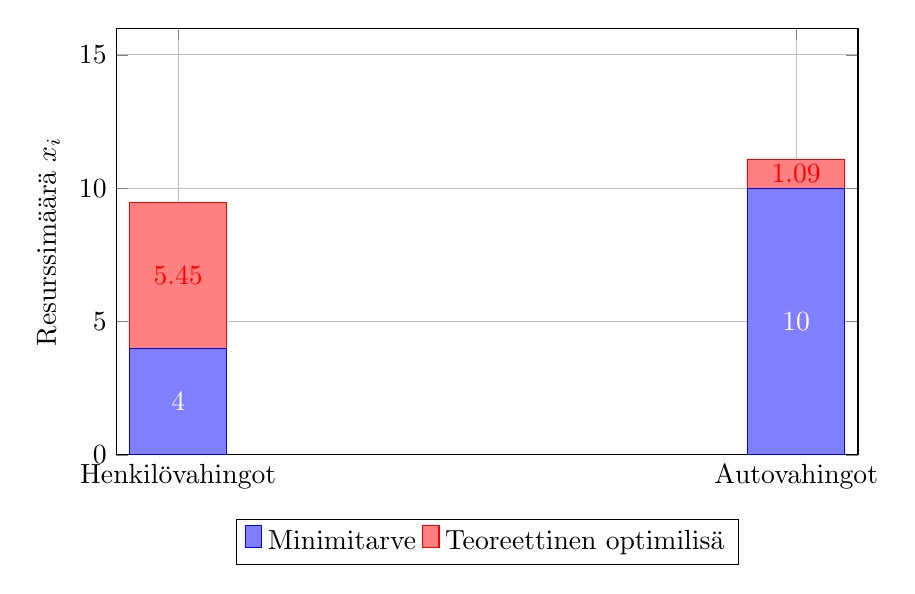
\begin{tikzpicture}
\begin{axis}[
    ybar stacked,
    width=11cm, height=7cm,
    ymin=0, ymax=16,
    symbolic x coords={Henkilövahingot, Autovahingot},
    xtick=data,
    ylabel={Resurssimäärä $x_i$},
    legend style={at={(0.5,-0.15)}, anchor=north, legend columns=-1},
    grid=major,
    bar width=35pt,
    nodes near coords,
    nodes near coords align={center},
    point meta=rawy, % Käyttää y-arvoja suoraan
    /pgf/number format/.cd, fixed, precision=2 % 2 desimaalia
]
    % Pakollinen osa
    \addplot+[fill=blue!50, text=white] coordinates {(Henkilövahingot, 4) (Autovahingot, 10)};
    \addlegendentry{Minimitarve}

    % Optimilisä
    \addplot+[fill=red!50] coordinates {(Henkilövahingot, 5.45) (Autovahingot, 1.09)};
    \addlegendentry{Teoreettinen optimilisä}
    
\end{axis}
\end{tikzpicture}
\end{center}









\end{document}